% !TEX root = ../main.tex
%
\chapter{Related Work}
\label{sec:related}

% Overview (free-by-me) READY
Before describing the problem, and later on the experimental setup, we first
\begin{enumerate}
    \item Revise three common prediction tasks in \acp{gnn}
    \item Give a general overview of how \acp{gnn} organize and process graph structured data
    \item We further discuss the relation of messasge passing mechanis to the \ac{wl}, an algorithm for
          inspecting wheather two graphs are isomorph.
    \item Give an formal definition and description of two \ac{gnn}
          architectures, which will be used in our experiments.
\end{enumerate}


\section{Prediction Tasks and Typical Problems}
\label{sec:related:pred}

% Types of prediction tasks (free-by-me) READY
Graphs naturally appear in numerous application domains, ranging from social analysis,
bioinformatics to computer vision.
A Graph $G = (V,E)$, where $V = \{v_{1},...,v_{n}\}$ is a set of $N =|V|$ nodes and
$E \subseteq V\times V$ a set of edges betwen those nodes. The unique capability of
graphs enables capturing the structural relations among data, and thus allows to harvest more
insights compared to analyzing data in isolation~\cite{Zhang19}. Graphs therefore can be
seen as a general laguage for describing entities and relationships between those entities.
\Acfp{gnn} then organize graph structured data to tackle various prediction and classification
tasks. Typically, one is interested in one of the following three tasks:
\begin{enumerate}[label=\textbf{\arabic*.}]
    \item \textbf{Link prediction:}
          Predict whether there are missing links between two nodes
          e.g., knowledge graph completion

    \item \textbf{Vertex classification \& regression:}
          Predict a property of a node e.g., categorize online users/items

    \item \textbf{Graph classification \& regression:}
          Here we are interested in classifying or predicting a continous value for
          the entire graph e.g., predicting a property of a molecule.
\end{enumerate}

In this work the main focus will be on the latter two, \ac{nc}\ \ac{nr} and \ac{gc}\
\ac{gr} for small- as well as large-sized graphs.

% Message passing formally
\section{Passing Messages in \Acsp*{gnn}}
\label{sec:related:message}

% Intro to GNNs, State-description (free-by-me) READY
Graphs, by nature are unstructured. Vertices in graphs have no natural order and can
contatin any type of information. In order for machine learning algorithms to be able
to make use of graph structured data, a mechanism is needed to organize them in a
suitable way.
\cite{Zhou2020a}
\cite{Hamilton2017a}
\cite{Zhang19}


% Message Passing in general (free-by-me) READY
Message passing is a mechanism~\cite{Xu2019}~\cite{Zhou2020a}, which embedds into every node information about it's neighbourhood.
This can be done in several ways and one way of classifying a \ac{gnn} is by looking at the
underlying message passing machanism. In this paper we will look at a network, where message passing is done
via convolutions (\acf{gcn}). We will however ocasionally use the more general term message passing, as
the separation is rather blurred and message passing is seen as a generalization of
other, more specific mechanisms

Formally, message passing in a \ac{gnn} can be described as using two functions:
AGGREGATE and COMBINE. The expressive and representational power of a \ac{gnn} can
then be determined by looking at the concrete functions and thier properties, used to implement
aggregation and combination. AGGREGATE mixes in every iteration the hidden representation of the node
with the representation of nodes neighbourhood. COMBINE then combines the mixed representation togheter with the
representation of the node. Each node uses the information from its neighbors to update its embeddings, thus a natural
extension is to use the information to increase the receptive field by performing AGGREGATE and COMBINE multiple
times.

\begin{align*}
    a_{v}^{k} = \mathrm{AGGREGATE}^{(k)}(\{h_{u}^{(k-1)}: u \in \mathcal{N}_{(v)}\}) , h_{v}^{(k)} = \mathrm{COMBINE}^{(k)}(h_{v}^{(k-1)}, a_{v}^{(k)})
\end{align*}

% Message passing framework and local graph structure (free-by-me) READY
One useful type of information, which the message passing framework should be able to
capture, is the local graph structure. This can be done by choosing functions with
appropriate properties. A more detailed explanation will follow in
\cref{sec:related:architectures}. In spatial \ac{gnn} we make the assumption of the
similarity of neighbor nodes. To exploit this spatial similarity, we perform
composition by stacking multiple layers togheter and increase the receptive field.

% picture of k-hop neighbourhood aggregation (free-by-me) READY
\begin{figure}[ht]
    \centering
    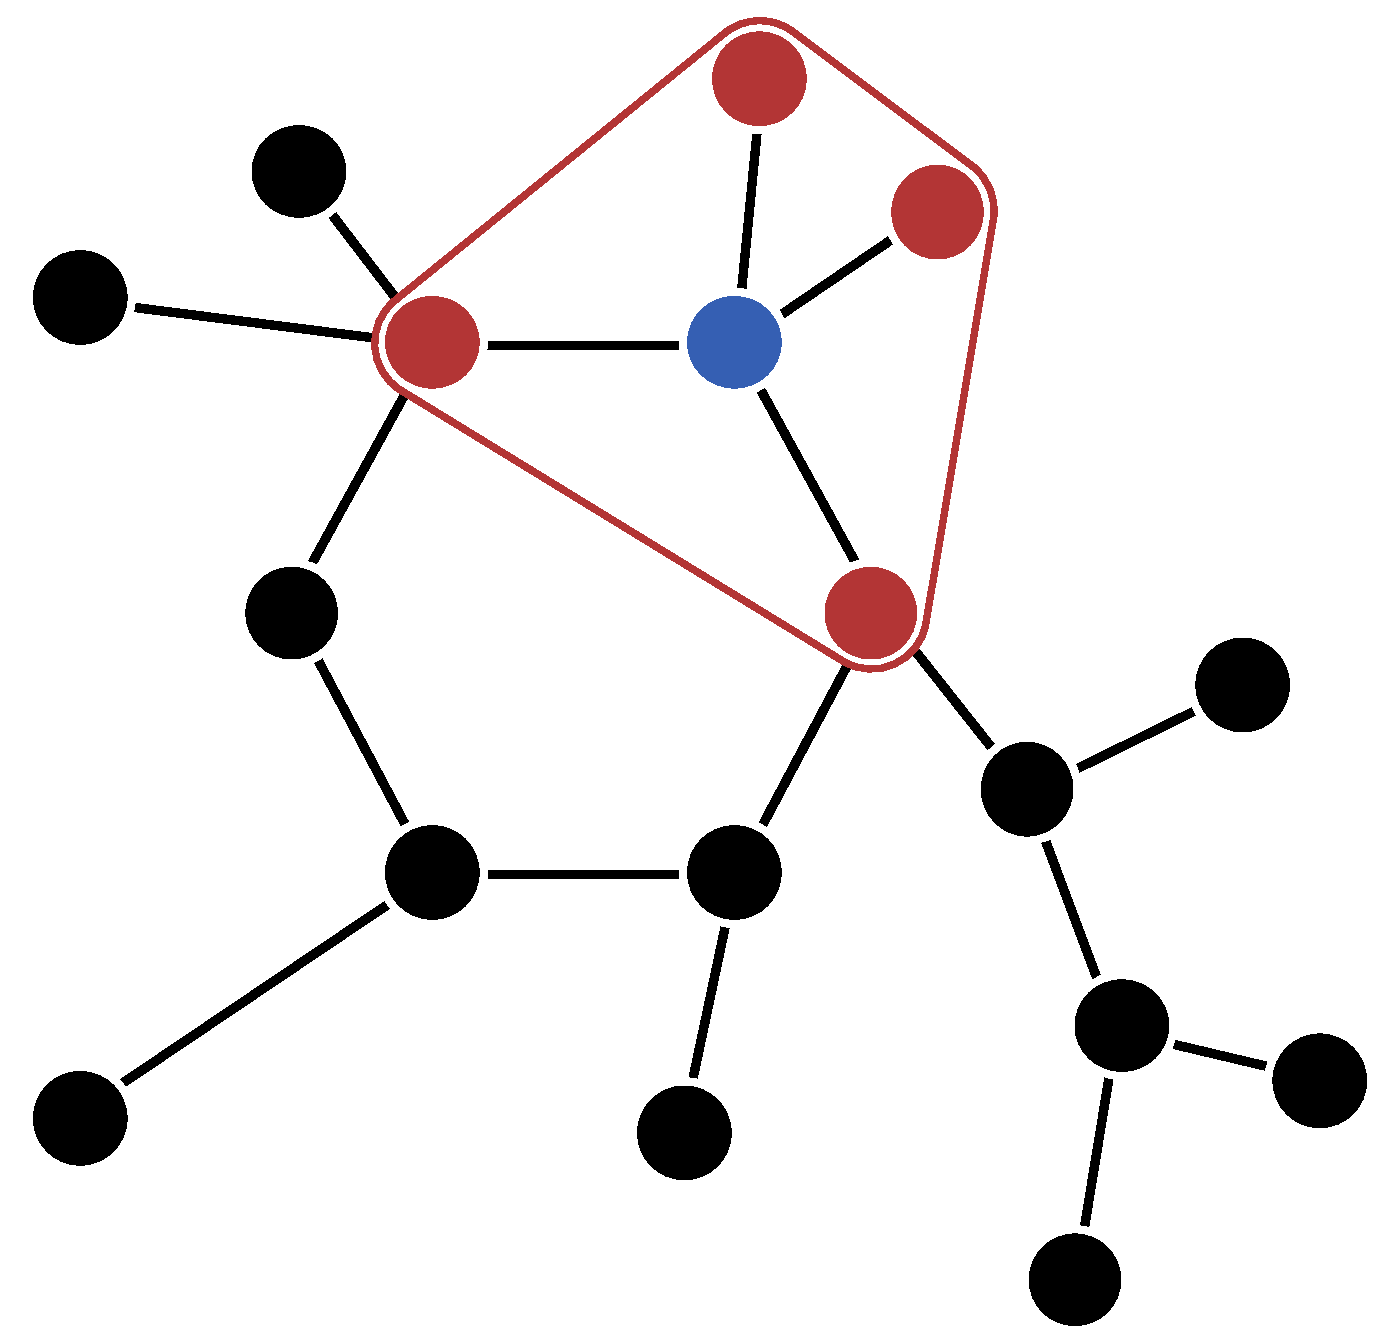
\includegraphics[width=0.35\linewidth]{gfx/related-work/1hop}\hspace{1cm}
    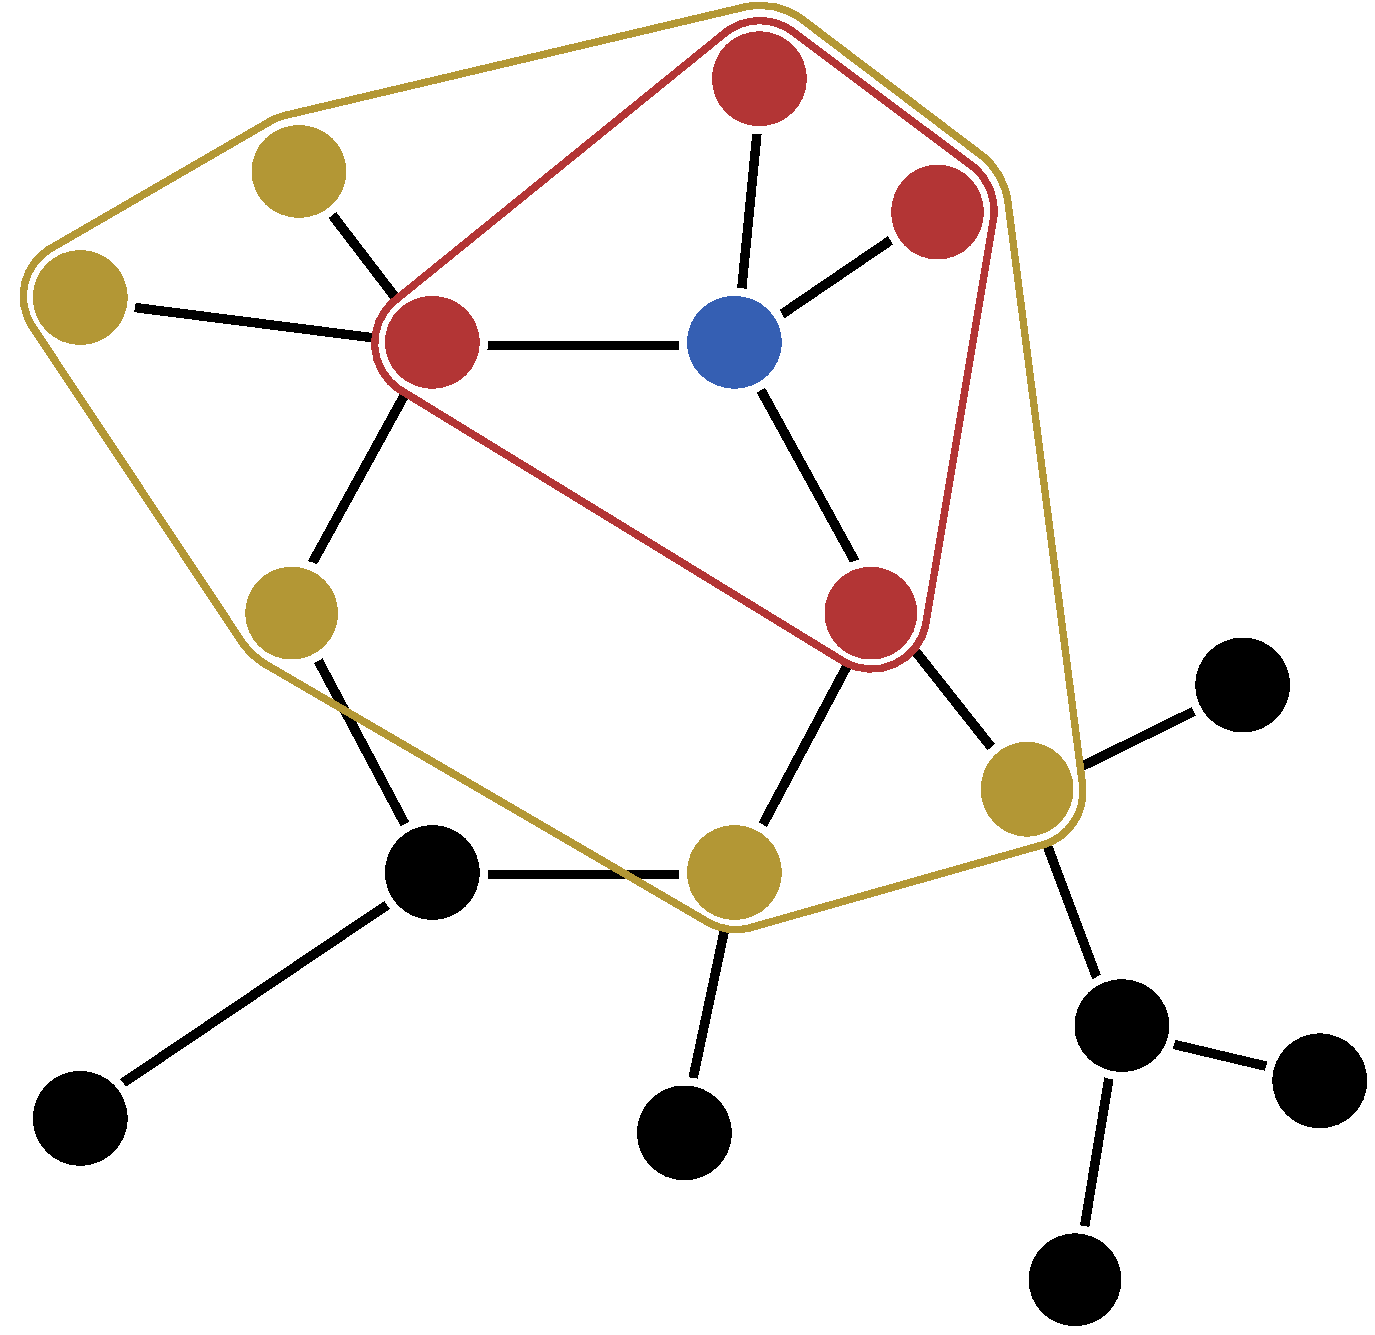
\includegraphics[width=0.35\linewidth]{gfx/related-work/2hop}
    \caption{By performing aggregation k-times we can reach the k-hop neighborhood}\label{fig:related:1hop}
\end{figure}


\subsection{\acl{wl} Graph Colorings}
\label{sec:related:character:wl}
% What is the Weisfeiler lehman test 
% Definition and relation to neural networks 
The Message passing mechanism has a close relation, to the way the \acf{wl} test ~\cite{Weisfeiler1968}
~\cite{Damke2020}~\cite{Huang2022}, an algorithm for deciding wheather two graphs are isomorphic works.

% Intro of Notations 
Before describing the \ac{wl} algorithm, we define preliminaries and introduce some notations.
% graph is defined in \sec 2.1 
\begin{defn}
    Let $G = (V,E)$ denote a graph where $V =\{v_{1},...,v_{n}\}$ is a set of $ N = |V|$
    nodes and $E \subseteq V\times V $ a set of edges between those nodes.
\end{defn}

% The 1-WL in it's one-dimensional form 
\subsubsection{The 1-dimensional \acs{wl} algorithm (color refinement)}
In the 1-dimensional \ac{wl} algorithm (1-WL), a color is assigned to each vertex of a graph.
If the vertices $v \in \mathcal{V}_G$ of the input graph $G$ are labeled, those labels $l_G[v] \in L_{\mathcal{V}} \subseteq \mathcal{C}$ can be used as the initial graph coloring $\chi_{G,1}^{(0)}(v) \coloneqq l_G[v]$.
Since \ac{wl} colors are inherently discrete, continuous vertex feature vectors $x_G[v]$ are not considered here.
For unlabeled graphs a constant coloring is used, e.g.\ $\forall v \in \mathcal{V}_G: \chi_{G,1}^{(0)}(v) = \colorlabel{t_blue}{A}$ for some initial color $\colorlabel{t_blue}{A} \in \mathcal{C}$. % chktex 25
In each iteration of the 1-\acs{wl} color refinement algorithm, the following neighborhood aggregation scheme is used to compute a new color for each vertex:
\begin{defn}\label{defn:related:wl1-refine}
    $\chi_{G,1}^{(i+1)}(v) \coloneqq h\left(\chi_{G,1}^{(i)}(v), \ldblbrace \chi_{G,1}^{(i)}(u)\, |\, u \in \Gamma_{G}(v) \rdblbrace\right)$,
    with $\Gamma_G(v)$ denoting the set of adjacent vertices of $v \in \mathcal{V}_G$ and $h: \mathcal{C}^* \to \mathcal{C}$ denoting an injective hash function that assigns a unique color to each finite combination of colors.
\end{defn}
\begin{figure}[ht]
    \centering
    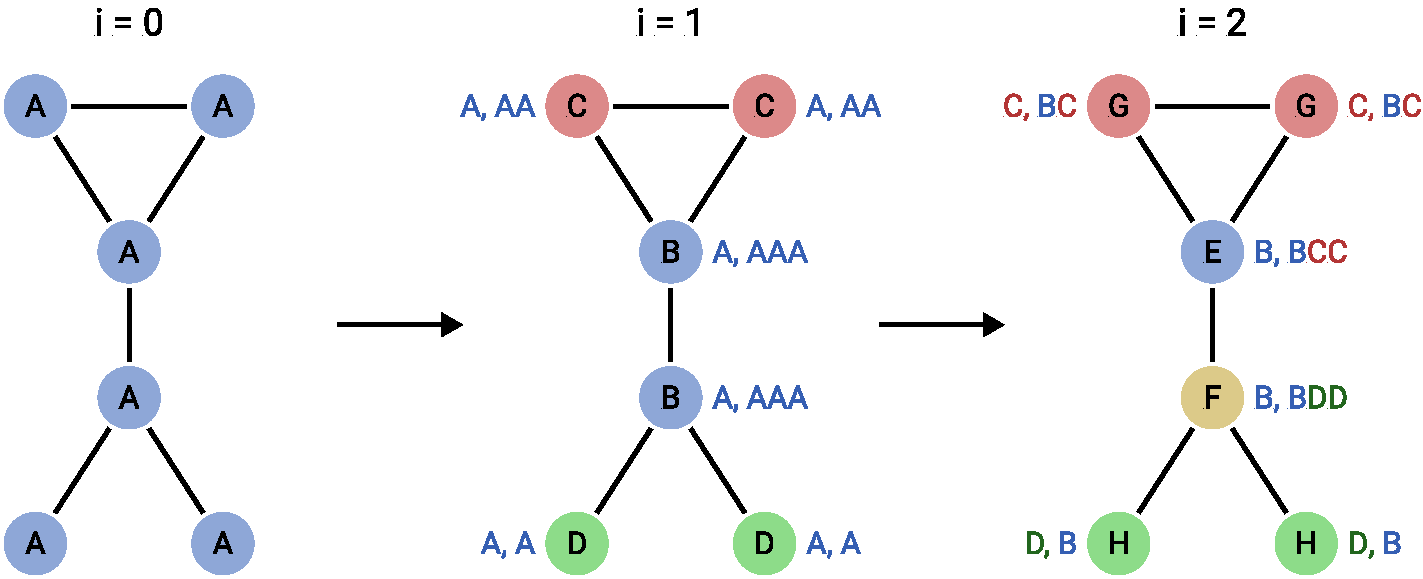
\includegraphics[width=0.72\linewidth]{gfx/related-work/wl1-refine.pdf}
    \caption[Example 1-WL color refinement steps.]{
        Example 1-WL color refinement steps.
        After two iterations the coloring stabilizes.
        Each vertex $v$ is labeled with its current color and has its previous color and the colors of the hashed neighbors $\Gamma_G(v)$ written next to it (see \cref{defn:related:wl1-refine}).
    }\label{fig:related:wl1-refine}
\end{figure}

% How does the WL test perform 
The \acf{wl} algorithm characterizes a graph $G$ by assigning discrete labels $c \in \mathcal{C}$, called \textit{colors}, to vertex $k$-tuples $(v_1, \dots, v_k) \in \mathcal{V}_G^k$, where $k \in \mathbb{N}_0$ is the freely choosable \textit{\ac{wl}-dimension}.
A mapping $\chi_{G, k}: \mathcal{V}_G^k \to \mathcal{C}$ is called a \textit{$k$-coloring} of $G$.
\begin{defn}
    A coloring $\chi'$ \textit{refines} $\chi$ ($\chi' \preceq \chi$) iff.\ $\forall a, b \in \mathcal{V}_G^k: \chi(a) \neq \chi(b) \rightarrow \chi'(a) \neq \chi'(b)$, i.e.\ $\chi'$ distinguishes at least those tuples that are distinguished by $\chi$.
\end{defn}
\begin{defn}
    Two colorings $\chi$ and $\chi'$ are \textit{equivalent} ($\chi \equiv \chi'$) iff.\ $\chi \preceq \chi' \land \chi \succeq \chi'$, i.e.\ $\chi$ is identical to $\chi'$ up to color substitutions.
\end{defn}
The $k$-dimensional \ac{wl} algorithm ($k$-\acs{wl}) works by iteratively refining $k$-colorings $\chi_{G, k}^{(0)} \succeq \chi_{G, k}^{(1)} \succeq \dots$ of a given graph $G$ until the convergence criterion $\chi_{G, k}^{(i)} \equiv \chi_{G, k}^{(i+1)}$ is satisfied.
We denote the final, maximally refined $k$-\acs{wl} coloring with $\chi^{*}_{G, k}$.
\begin{defn}
    The color distribution $\mathit{dist}_{\chi_{G, k}}: \mathcal{C} \to \mathbb{N}_0$ of a $k$-coloring $\chi_{G, k}$ counts each color $c \in \mathcal{C}$ in the coloring, i.e.\ $\mathit{dist}_{\chi_{G, k}}(c) \coloneqq \left|\left\{ v \in \mathcal{V}_G^k\, |\, \chi_{G, k}(v) = c \right\}\right|$. % chktex 21
\end{defn}
\begin{defn}\label{defn:related:wl-distinguishable}
    Two graphs $G$ and $H$ are $k$-\acs{wl} \textit{distinguishable} ($G \mathrel{{\not\simeq}_k} H$) iff.\ there exists a color $c \in \mathcal{C}$ s.t.\ $\mathit{dist}_{\chi^{*}_{G, k}}(c) \neq \mathit{dist}_{\chi^{*}_{H, k}}(c)$.
\end{defn}
As we will see, the way in which \ac{wl} colorings are refined is vertex order invariant;
thus any difference in the final coloring of two graphs always implies the non-isomorphism of the colored graphs, i.e.\ $G \mathrel{{\not\simeq}_k} H \implies G \not\simeq H$.
The opposite does however not necessarily hold;
two $k$-\acs{wl} indistinguishable graphs are not always isomorphic, i.e.\ $\exists\, G, H: G \mathrel{{\simeq}_k} H \land G \not\simeq H$. % chktex 21

In addition to the binary aspect of \ac{wl} distinguishability and its relation to the \ac{gi} problem, \ac{wl} colorings are also useful for more fuzzy graph similarity comparisons as we will see in \cref{sec:related:pred:regularization} when we look at graph kernels.
Before that however, the details of the \ac{wl} color refinement strategy have to be described.
We begin with the color refinement algorithm for the most simple case of $k = 1$.
Then the definitions and intuitions from the 1-dimensional case are extended to its higher-dimensional generalization.
Lastly we will discuss the discriminative power of the \acs{wl} algorithm and its relation to the \acs{wl}-dimension $k$.


\subsection{GNN Architectures in this Paper}
\label{sec:related:architectures}

Experiments will be conducted on two types of \acp{gnn}: \ac{gcn} and \ac{gin}



\subsubsection{Graph Convolutional Network (GCN)}
\label{sec:related:architectures:gcn}
Graph Convolutional Network \ac{gcn} as proposed by the authors \cite{Kipf2017} has the
following layer-wise propaation rule

\begin{align*}
    H^{(l+1)} = \sigma (\tilde{D}^{-\frac{1}{2}}\tilde{A}\tilde{D}^{-\frac{1}{2}} H^{(l)}W^{(l)})
\end{align*}


% \cref eq 
and is very broadly used for a variety of different tasks, such as for instance node Classification tasks.
Despite not being as powerful as the \ac{gin} architecture, this architecture is sufficient for a lot
of tasks, especially when there is no need for distinguishing different structures/ substructures
of a graph and the prediction can be done with.

The authors claim, the model scales linearly in the number of graph edges and learns hidden layer
representations that encode both local graph structure and features of nodes.

\subsubsection{Graph Isomorphism Network (GIN)}
\label{sec:related:architectures:gin}
To overcome the lack of expressivity of popular GNN architectures,
Xu et al. designed a new type of \ac{gnn}, the graph isomorphism network \ac{gin}. They proved that
\acp{gin} are strictly more expressive than a variety of previous GNNs and that they are in fact
as powerful as the commonly used Weisfeiler-Lehman graph isomorphism test.

The key idea is to use injective functions, so that the function would never map two different
neighbourhoods to the same representations. \cite{Xu2019}

The following layer- wise propagation rule shows a forward pass in a \ac{gin}

\begin{align*}
    h^{(k)}_{v} & = \mathrm{MLP}^{(k)} ((1 + \epsilon^{(k)}) *h^{(k-1)}_{v} + \sum_{{u} \in{\mathcal{N}(v)}} \,h^{(k-1)}_{u} \\
    x           & = \mathcal{A}: \mathcal{G} \rightarrow\mathbb{R}^{d}
\end{align*}





Assuming, that the following conditions hold, with a sufficient number
of \ac{gnn} - layer A is as powerful as the \ac{wl} Test




\subsection{Weaknesses and Obstacles in \ac{gnn} Architectures}
\label{sec:related:pred:typical}
% What are the typical problems in GNNs (free-by-me) READY
Because of the way \acp{gnn} operate, they tend to suffer from two main obstacles:
overfitting and oversmoothing.

% Overfitting description and intuition 
Overfitting hinders the generalization ability of a \acf{nn}, making it perform poorly
on previously unseen data. This problematic occurs expecially when using small datasets,
since the model thends to 'memorize' instead of learn the pattern.


% Oversmoothing description and intuition (free-by-me) READY 
Oversmoothing is a condition, where the performance and predictive power of a \ac{nn}
does not imporve of even gets worse when more layers are added. This happens because
by stacking multiple layers  togheter togheter aggregation is being performed over and over again.
This way, the representation of a node is being smoothed - mixed with features of
very distant, possibly unrelated nodes. Oversmoothing is a problem mainly for node classification
tasks. There is a trade-off between the expressivness of the model (capturing) graph structure by
applying multiple layers and oversmoothing, which leads to a model where nodes have the same representation,
because they all converge to indistinguishable vectors.\cite{Zhou2020}\cite{DBLP:journals/corr/abs-2006-04064}
(In spatial \acp{gnn} we make the assumption of relatedness by proximity)


% Why is this happening (free-by-me) READY 
A closer examination of underlying causes of oversmoothing was conducted by \cite{Chen2020},
who suggested, that not message passing itself, but the type of interacting nodes cause this issue.
For \acf{nc} tasks, intra-class communication (interaction between two nodes sharing the same class)
is useful (signal), whereas inter-class communication (the communication between two nodes sharing
different lables) is considered harmful, because it brings interference noise into the
feature-representations by mixing unrelated features and therefore making unrelated nodes more similar
to each other. Because of that, the the quality of shared information is essencial and should
therefore be considered as a benchmark for improvement.



% THOSRE ARE MAIN TWO OBSTACLES I WILL FOCUS ON 
% HERE ARE SOME OTHER THINGS POSSIBLY TO CONSIDER LATER 
% https://www.blopig.com/blog/2021/10/issues-with-graph-neural-networks-the-cracks-are-where-the-light-shines-through/


\subsection{Regularization Techniques}
\label{sec:related:pred:regularization}

% What is Ragularization generally? 
\cite{Kukacka2017} define Regularization as any supplementary technique that aims at making the
model generalize better, i.e. produce better results on the test set, which can include various
properties of the loss function, the loss optimization algorithm, or
other techniques.

% Classification of reg.t -> stochastic regularization 

One subgroup of regularization is via data, where the training set $\mathcal{D}$ is
transformed into a new set $\mathcal{D}_{R}$ using some stochastic parameter
$\theta$, which can be used in various ways, including to manipulate the feature space,
create a new, augmented dataset or to change (e.g, thin out the hidden layers of
the \ac{nn})

% What types of problems does it solve? Relation ty my specific subset (overfitting, oversmoothing in GNNs)

In the scope of this work we will look at various regularization techniques
and thier efficacy in terms of dealing with the issues of overfitting and oversmoothing
The four regularization approaches, as described by \cite{DBLP:journals/corr/abs-2006-04064} are:

% Detailed description of techniques 

\ac{do}\\
\ac{do} randomly removes elements of its previous hidden
layer $H^{(l)}$ based on independent Bernoulli random draws
with a constant success rate at each training iteraration: \cite{DBLP:journals/corr/abs-2006-04064}
\begin{align*}
    H^{(l+1)} = \sigma(\mathfrak{R}(A)(Z^{(l)}\odot H^{(l)}) W^{(l)})
\end{align*}


Originally this method was proposed by \cite{Srivastava2014}, who proposed to
randomly drop units (along with their connections) from the neural
network during training and thus prevent units from co-adapting too much.
During training dropout samples from an exponential number of different "thinned" networks.At
test time, it is easy to approximate the effect of averaging the predictions of all these thinned networks
by simply using a single unthinned network that has smaller weights. This signifcantly
reduces overftting and gives major improvements over other regularization methods.


Exspecially when working with small datasets we have much noize, which then leads the model
to overfit.
\ac{de}

\begin{align*}
    H^{(l+1)} = \sigma(\mathfrak{R}(A \odot Z^{(l)}) H^{(l)} W^{(l)})
\end{align*}



\ac{ns}
\begin{align*}
    H^{(l+1)} = \sigma (\mathfrak{R}(A) diag(z^{(l)}) H^{(l)} W^{(l)})
\end{align*}



\ac{gdc}
\begin{align*}
    H^{(l+1)}[:,j] = \sigma (\sum_{i=1}^{f_{t}}\mathfrak{R}(A \odot Z_{i,j}^{(l)})H^{(l)}[:,i]W^{(l)}[i,j])
\end{align*}

% Intuition and pittfalls 

\section{Conclusion}
\label{sec:related:conclusion}
% this is for me for now 
\acp{gnn} are widely used. They make use of a mechanism called message passing, which
is done specifically by using two functions AGGREGATE and COMBINE.
The concrete choice of these functions determines the type of \ac{gnn}
and it's expressive power. If we want the network to have the same expressive
and representational as the \ac{wl}, the functions need to be injective in order
to map different neighbourhoods to different representations.

Also, since graphs have no natural order, the functions need to be permutation
invariant.


There are three typeical prediction tasks in \acp{gnn}, two of which we will concider
in this work. (We focus on node classification\ regression as well as
graph classification\ regression)